\documentclass{article}
\usepackage{graphicx} % Required for inserting images

\usepackage{graphicx} % Required for inserting images
\usepackage[utf8]{inputenc}
\usepackage{graphicx}
\usepackage{wrapfig}
\graphicspath{ {./images/} }
\usepackage{graphicx}
\usepackage{wrapfig}
\usepackage{float}
\usepackage{graphicx}
\usepackage{subcaption}
\usepackage[export]{adjustbox}
\usepackage{wrapfig}
\usepackage{blindtext}
%Image-related packages
\usepackage{graphicx}
\usepackage{subcaption}
\usepackage[export]{adjustbox}
\usepackage{wrapfig}

\title{Computational Simulation of the Behaviour of the 5 Inner Planets of the Solar System}
\author{Guilherme Garcia \\ s2240769 \\ The University of Edinburgh \\ School of Physics and Astronomy}
\date{April 2023 }



\begin{document}

\maketitle

\section{Introduction}

{The main goal of this project was to create a simulation that presents a good approximation of the working of the 5 innermost planets of the Solar System. This was achieved by computationally simulating the solar system and then performing different experiences on the system to test the contribution of different factors to its working.}

{The experiments performed were:}

\begin{enumerate}
  \item Orbital Periods and Energy Conservation - Determining the Orbital period for each planet in the simulation and comparing them with the real values. Observing the total of the energy of the system trough a long period of time and confirm if it is conserved over time. 
  \item Influence of Jupiter on Inner Planets - Creating a system where the planets only feel the gravitational force from the Sun and are not affected by each other's gravitational pull and analyse how this affects the orbital periods of the 4 inner planets. 
  \item Direct Euler's Integration - Using Euler's method of integration (instead of Beeman's method) to compute the orbits of the planets and observe its effects on the orbital periods and the energy conservation of the system.
  \item Satellite to Mars - Simulating the launch of a satellite to Mars from Earth. This included finding the velocity for which the satellite gets closer to the planet and the time it takes to get there. The results were compared with previous missions to Mars in order to determine their accuracy.
  
\end{enumerate}

\section{Methods}

{The overall structure of the code is based on two types of different classes, a celestial bodies class that creates the planetary objects and the satellite which share the same attributes of position, mass and kinetic energy and an experiment class where the programs to perform each of the experiments run.}

{All experiments except from 3 use the Beeman integration method. In order to ensure it works the celestial bodies class has 2 different functions to update its characteristics one to update its position and one to update its velocity (that updates its acceleration inside it since the Beeman method uses 3 different accelerations). The velocities and positions of all the bodies in the simulation must be updated simultaneously in order to account for the effect of each body on one another.  }
\begin{figure}[H]
    \centering
    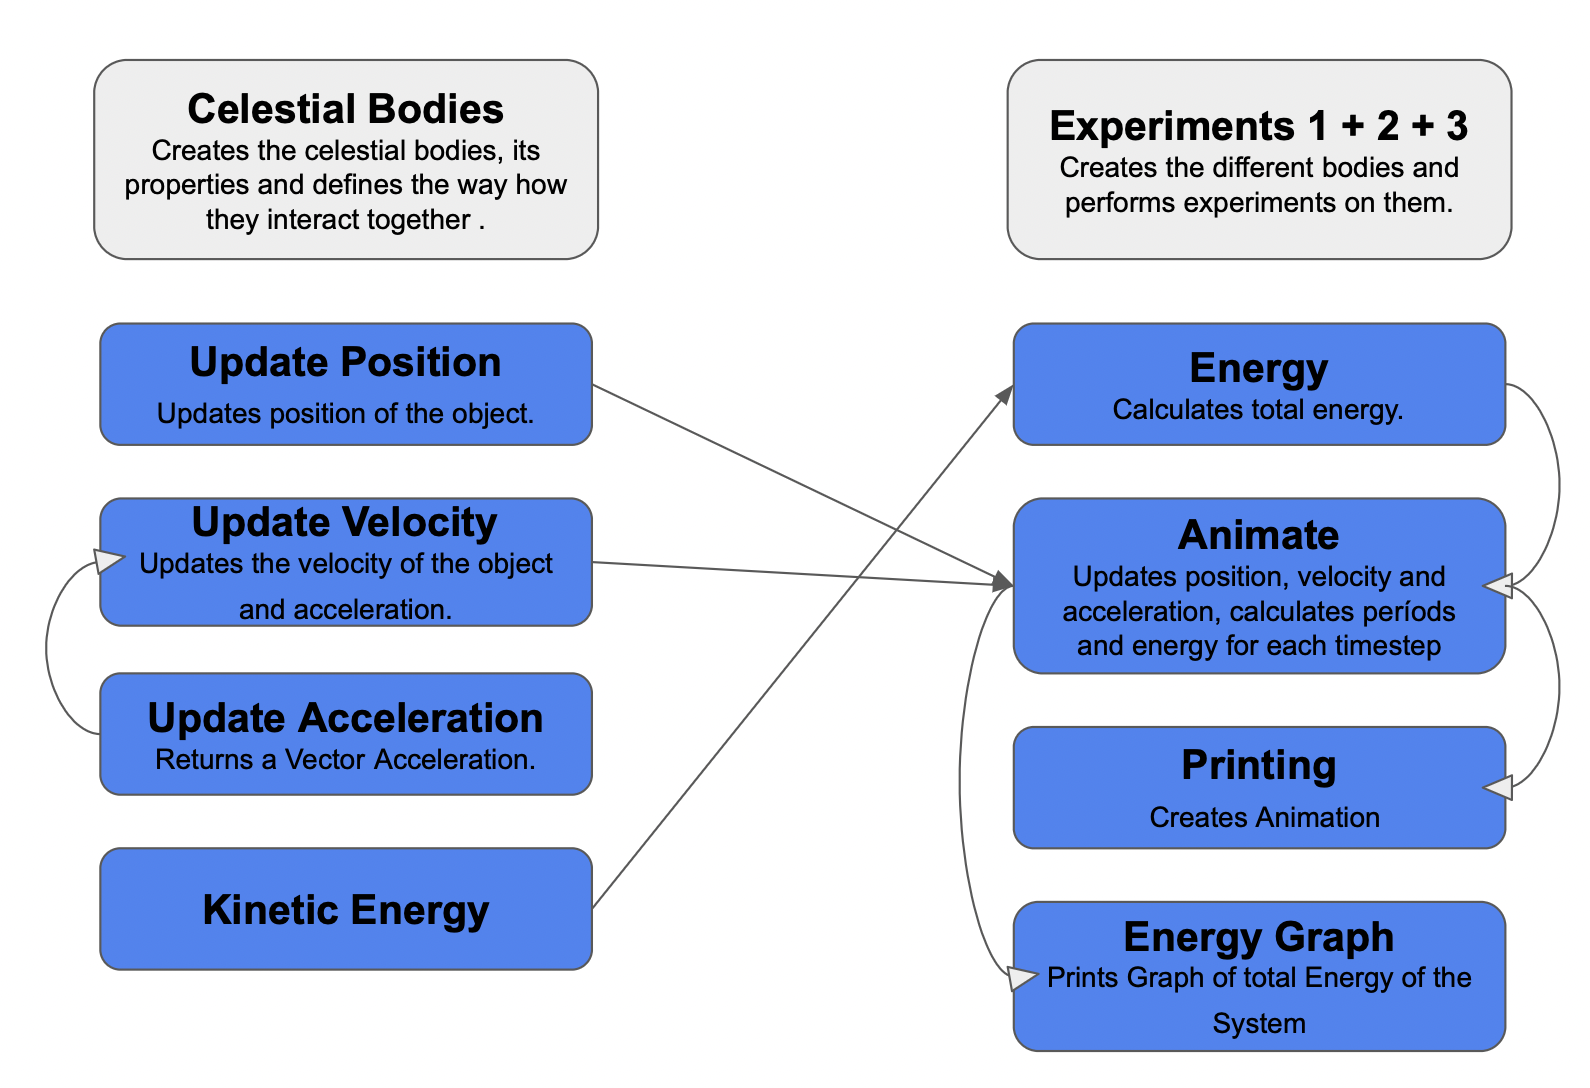
\includegraphics[width=11.115cm, height=7.455cm]{Experiment 1 .png}
    \caption{High-Level overview of the code for Experiment 1 and 2.}
    \label{fig:my_label}
\end{figure}
\subsection{Orbital Periods and Energy Conservation}

{Using the standard Beeman integration, a period was considered to be every time a planet passed the x-axis and an Earth year was considered to be 31557600 seconds. To calculate the energy of the system the kinetic energy of each planet and the potential energy of each pair of planets (in order to avoid double counting) were calculated for each time step and summed together (using the energy function). }

\subsection{Influence of Jupiter on Inner Planets}

To determine the effect of Jupiter on the Inner Planets orbital periods, a new Animate function was created where the planets' position, velocity and acceleration are only affected by the Sun and do not account for the gravitational pull of the other planets. This allowed for the computation of the periods of the planets due solely to the gravitational effect of the Sun only.
\subsection{Direct Euler's Integration}
\begin{figure}[H]
    \centering
    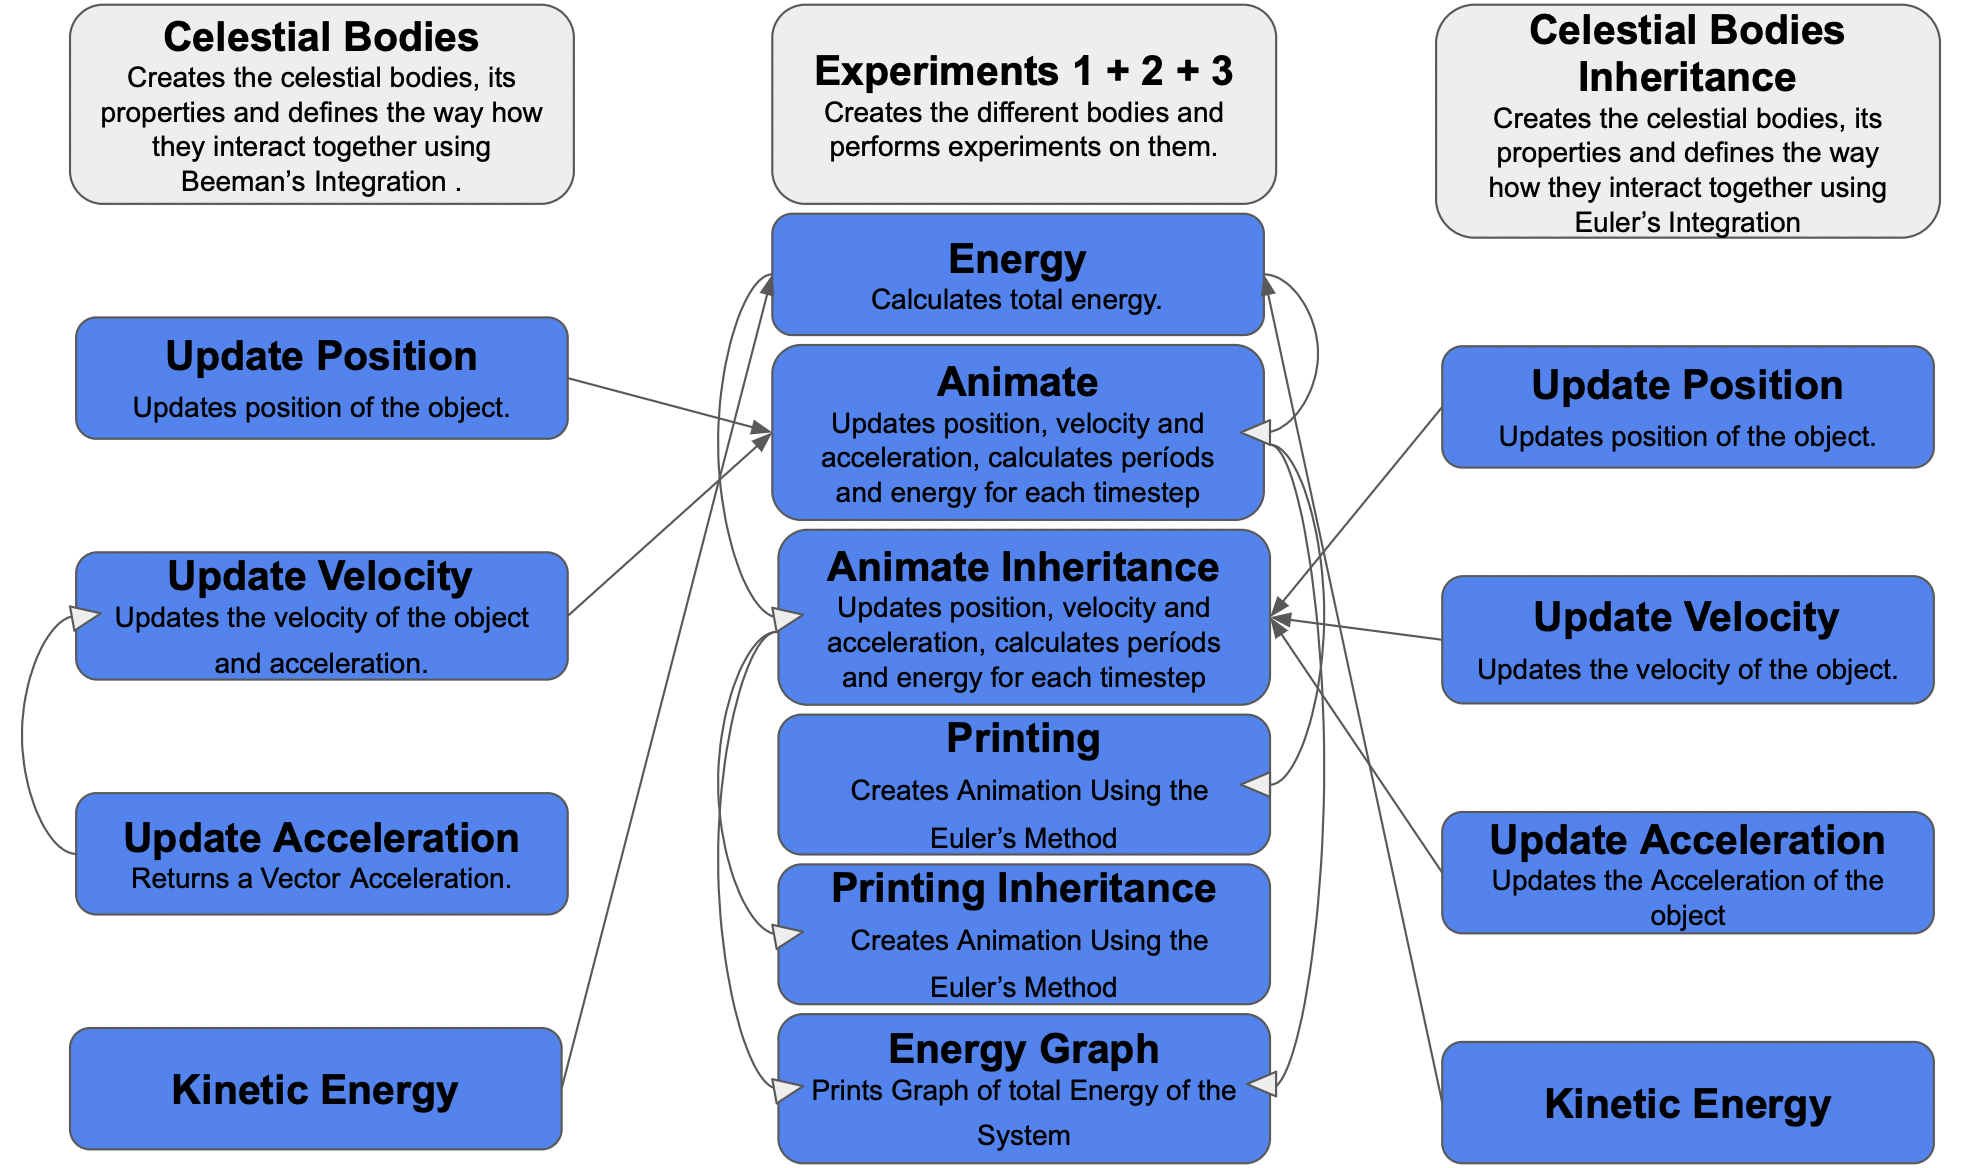
\includegraphics[width=11.856cm, height=7.008cm]{Experiment 3.png}
    \caption{High-Level overview of the code for Experiment 3.}
    \label{fig:my_label}
\end{figure}
{To determine the differences that the use of direct Euler's integration causes compared to Beeman's method, a new inherited celestial bodies class was created by reusing the code from checkpoint 5. Then 2 separate animations for the Solar System run and their energies through time are compared in order to determine the effect of the numerical integration method on energy conservation. }
\subsection{Satellite to Mars}

\begin{figure}[H]
    \centering
    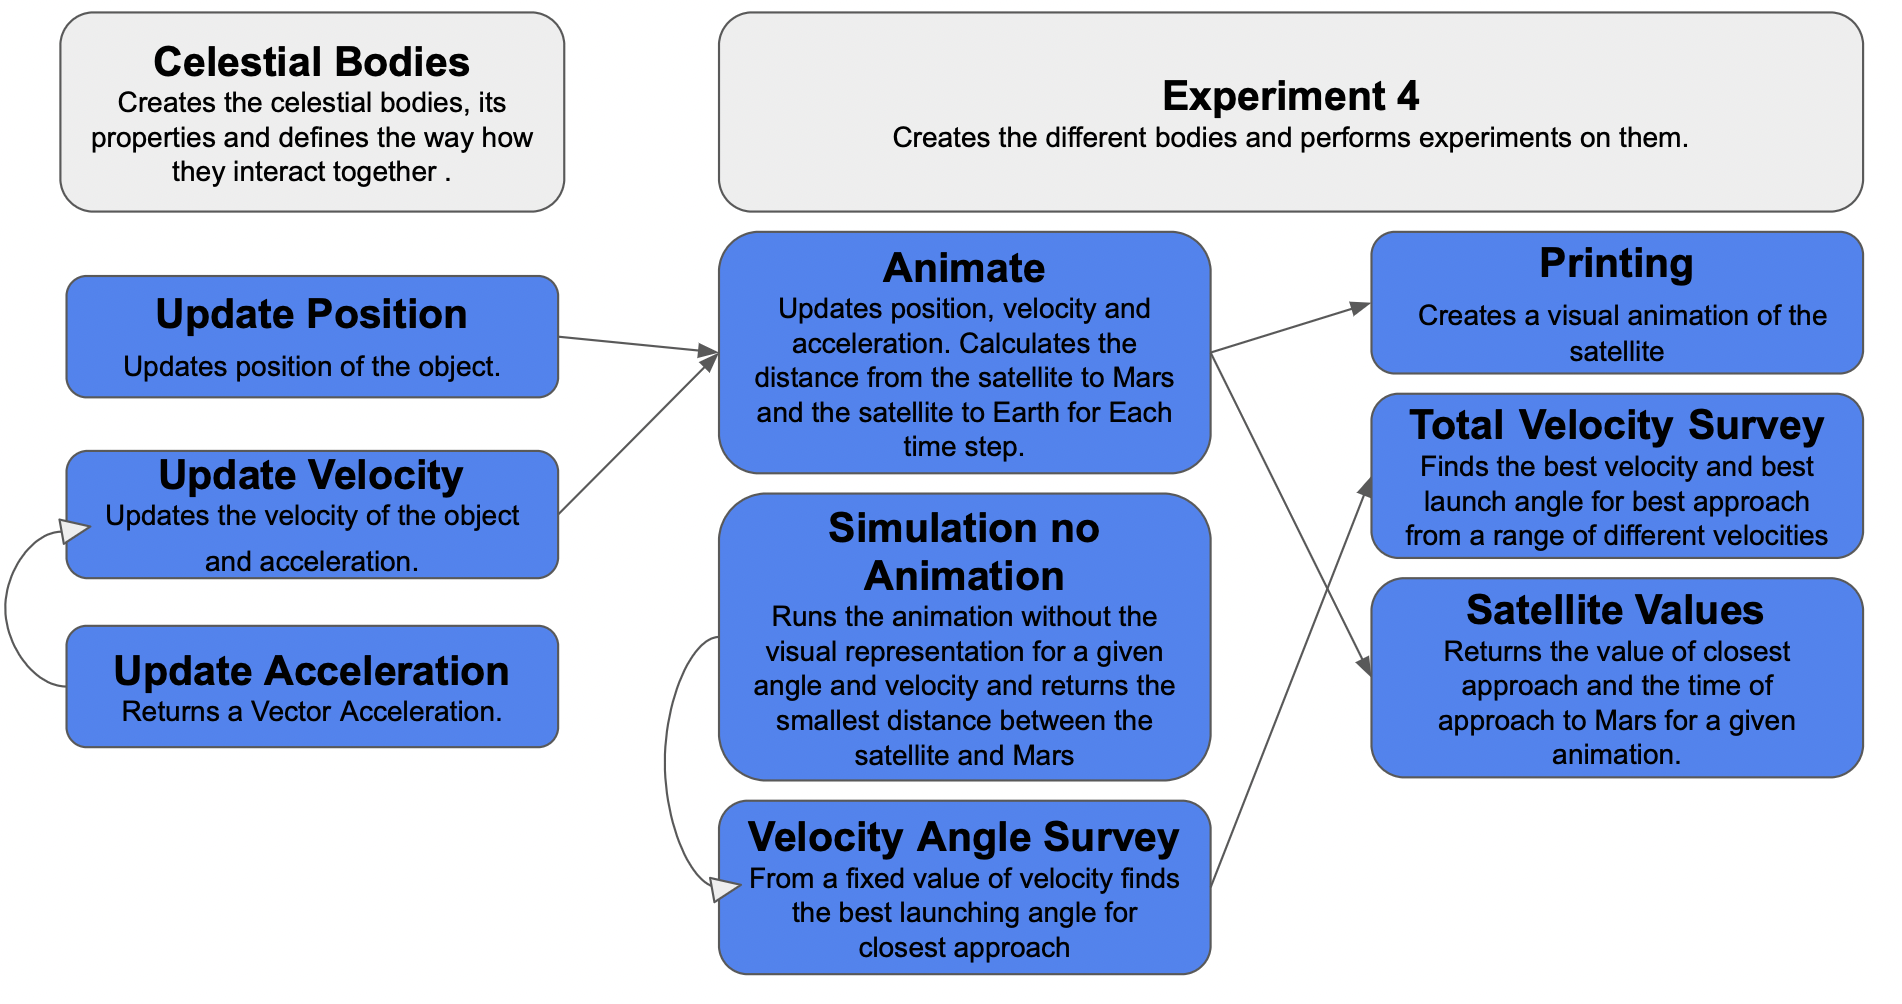
\includegraphics[width=11.412cm, height=6.024cm]{Experiment 4.png}
    \caption{High Level overview of the code for Experiment 4.}
    \label{fig:my_label}
\end{figure}

{To simulate the launch of a satellite from Earth to Mars a new experiment class was created in order to avoid overloading the previous class and make the code easier to read and understand.} {This simulation assumed a satellite orbiting $0.01Au$ above the Earth and with a mass of $1*10^{-21}$Earth-Masses. The orbit of this satellite can be considered to be approximately an Ohman transfer orbit[4] and as such, it is assumed that the satellite is orbiting the Earth that is revolving around the Sun, thus its initial velocity will be the same velocity with which the Earth orbits the Sun.}


{Firstly it was created a function that would allow the calculation of the optimal velocity and Angle of launch. This was done by creating a function that would calculate for a range of velocities launched at a range of different angles, the minimal distance with which the satellite would approach Mars for a given velocity modulus, returning, in the end, the velocity and angle of launch for which the distance to Mars is minimal.}

{Secondly, this velocity and Angle were plotted into an animation class that would allow for the calculation of the minimum distance of approach, the time of approach and the time of return to Earth. The time of return to Earth was found by having the function returning all the times for which the distance of the Satellite to Earth is less than $10^10$, distance at which the Satellite is considered to enter the Earth's orbit. This will happen in 2 instances, when the satellite is leaving Earth (which is ignored in the data analysis) and when the satellite returns, time which is used for the data analysis. }

{All these calculations need to be executed with a time step of 10000 seconds or inferior in order to get the most accurate results.}

\section{Results and Discussion}

\begin{figure}[H]
    \centering
    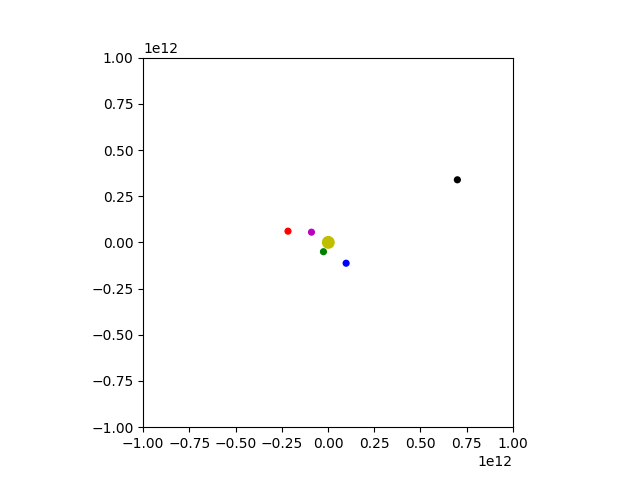
\includegraphics[width=11.115cm, height=7.455cm]{Solar Animation.png}
    \caption{Simulation of the Solar system.[1]}
    \label{fig:my_label}
\end{figure}

\subsection{Orbital Periods and Energy Conservation}

\begin{figure}[H]
    \centering
    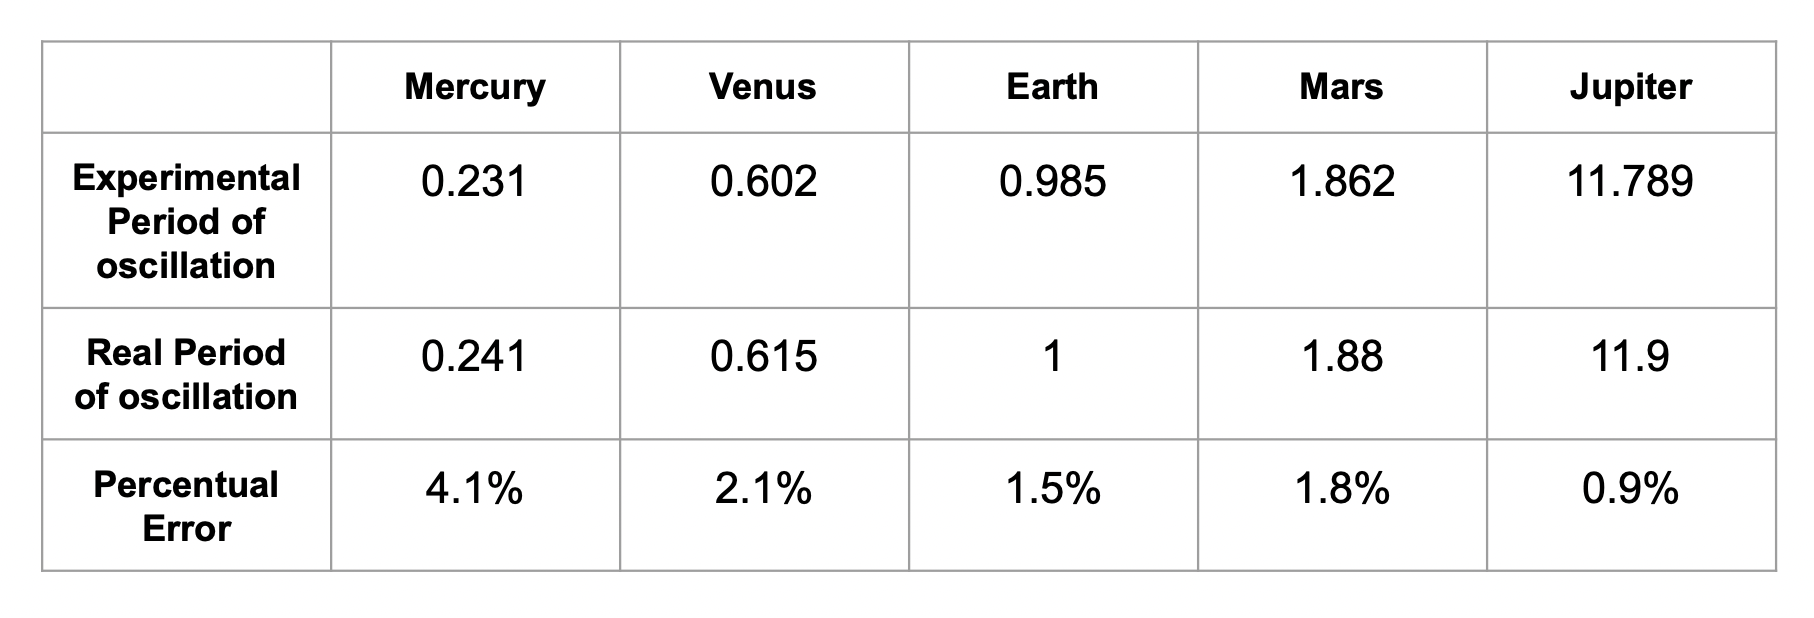
\includegraphics[width=13.0608cm, height=4.4496cm]{Errors.png}
    \caption{Comparison of Orbital Periods[1]}
    \label{fig:my_label}
\end{figure}

{As shown in Figure 5, the values of the orbital periods of the simulation have an orbital period within a $2\sigma$ level of the real values for the orbital periods with the average error for this calculation being $2.08\%$. The orbital period of Mercury has a bigger than average error which should be expected considering that since this simulation runs using classical mechanics and general relativity has a non-negligible effect on the orbit of Mercury[2].}

\begin{figure}[H]
    \centering
    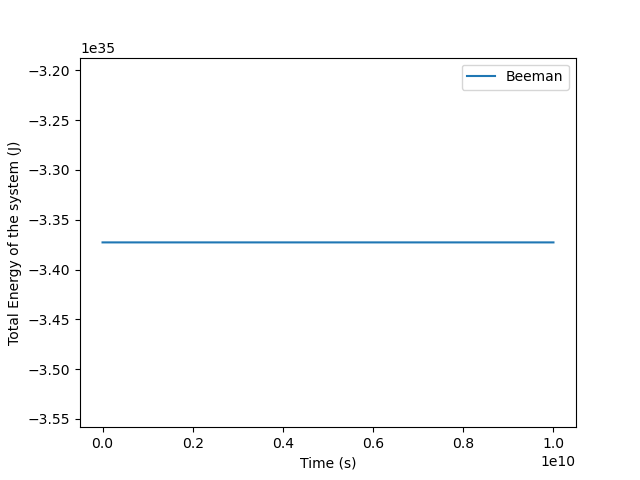
\includegraphics[width=7.68cm, height=5.76cm]{Beeman Eneergy conservation.png}
    \caption{Total Energy of the Solar System using Beeman Integration}
    \label{fig:my_label}
\end{figure}

{As shown in Figure 5 it is possible to state that when the simulation is left to run for about 300 years ($10^{10}$ seconds), the energy of the system is conserved). This is to be expected since the Solar System is treated as a closed system in this simulation and shows the adequacy of the Beeman integration method to describe the Solar System.}

\subsection{Influence of Jupiter on Inner Planets}

\begin{figure}[H]
    \centering
    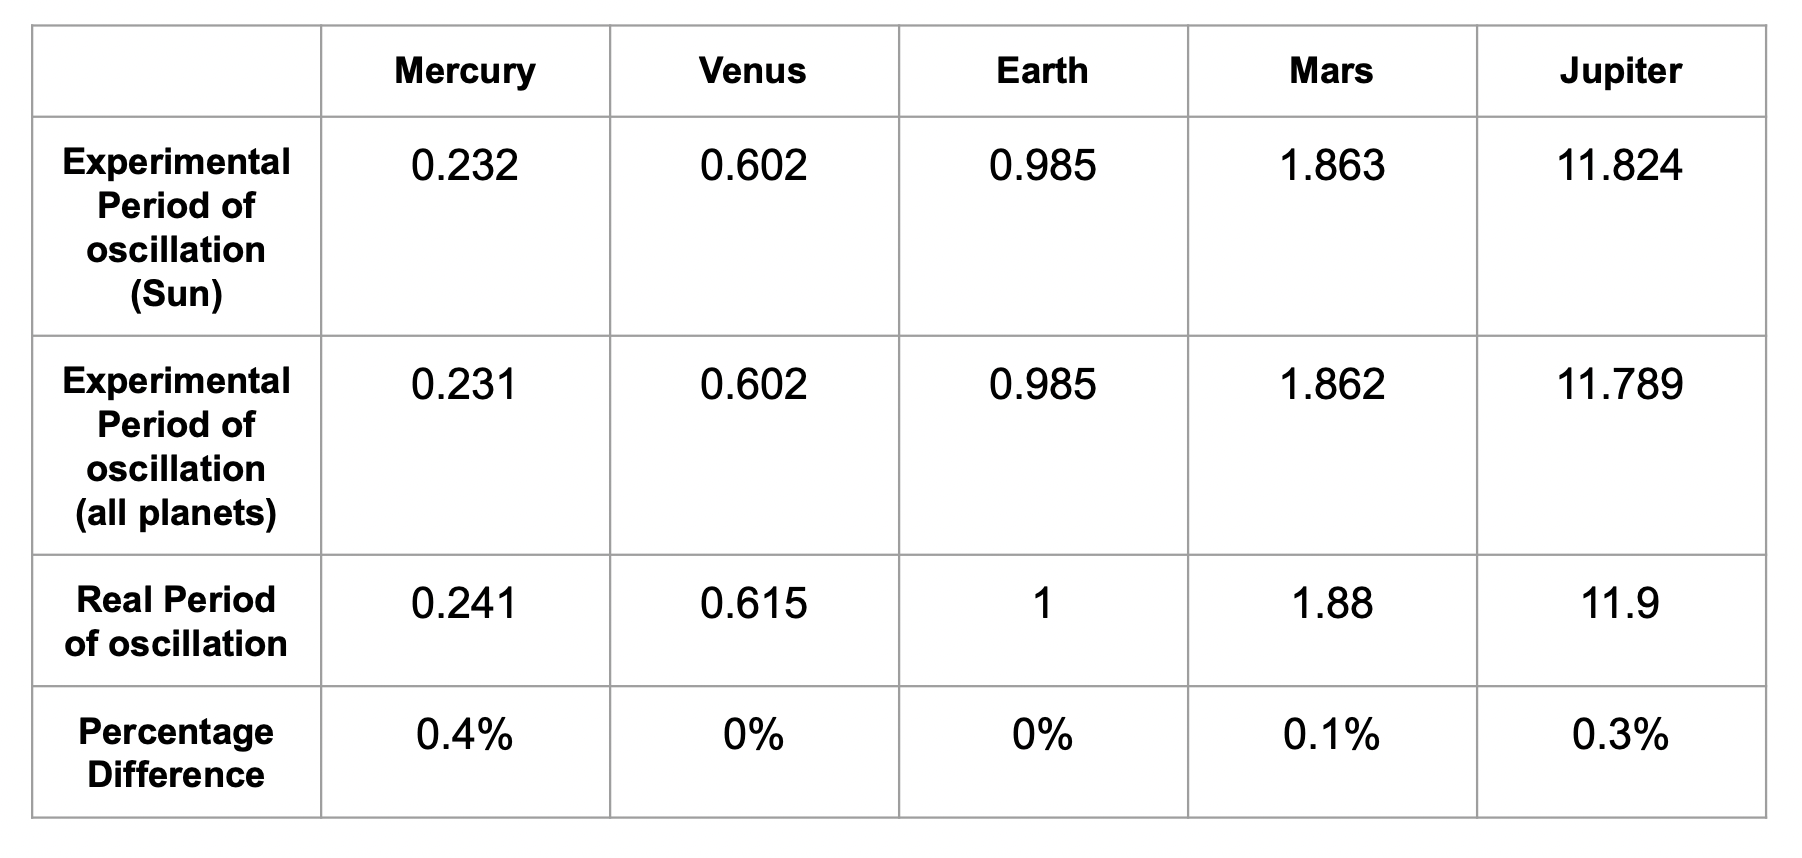
\includegraphics[width=12.614cm, height=6.006cm]{Sun Only.png}
    \caption{Orbital Periods of the planets for the case where all gravitational interactions are accounted for and for the case where only the Sun is considered.}
    \label{fig:my_label}
\end{figure}

{As shown in Figure 7 the effect of the other gravitational interactions of the inner planets is almost negligible in this experiment. This leads to the conclusion that for a small time frame (all these measurements were taken within 12 years of the beginning of the Simulation) the effects of Jupiter's Gravity on the inner planets can be neglected. However, we can easily understand that the small effect that this change may have on the planets will tend to compound over time thus the next step in this experiment would be to compute this simulation over a long time frame (300 years) and see what is its effect on periods.}

\subsection{Direct Euler’s Integration}

\begin{figure}[H]
    \centering
    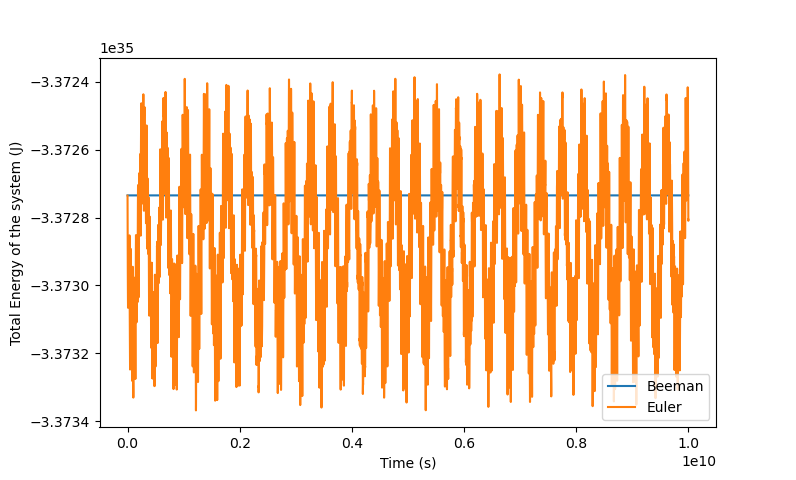
\includegraphics[width=7.96cm, height=4.80cm]{Euler Vs Beeman.png}
    \caption{Total Energy of the System using Euler's and Beeman's integration methods over approximately 300 years. }
    \label{fig:my_label}
\end{figure}

{As shown in Figure 8 the total energy of the system using the direct Euler's Integration is not as well conserved as with the Beeman's Integration. Thus,  allowing the conclusion that Beeman's Integration method will be preferable for simulations of the Solar System since one of its assumptions is that the Solar System is a closed system and its energy is conserved. }

\subsection{Satellite to Mars}

\begin{figure}[H]
    \centering

    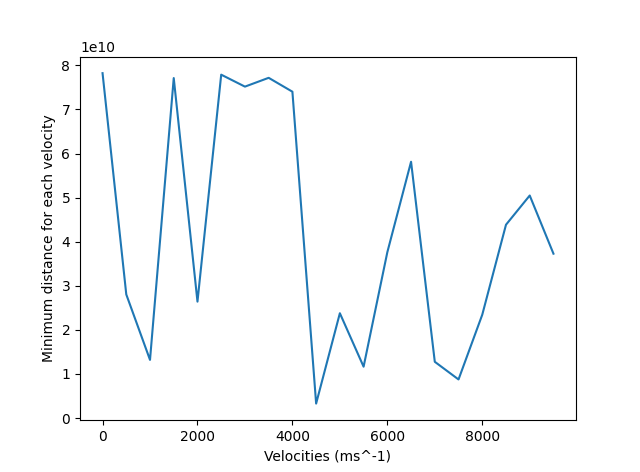
\includegraphics[width=6.40cm, height=4.80cm]{Long Range Velocities Survey - 9 degrees.png}


    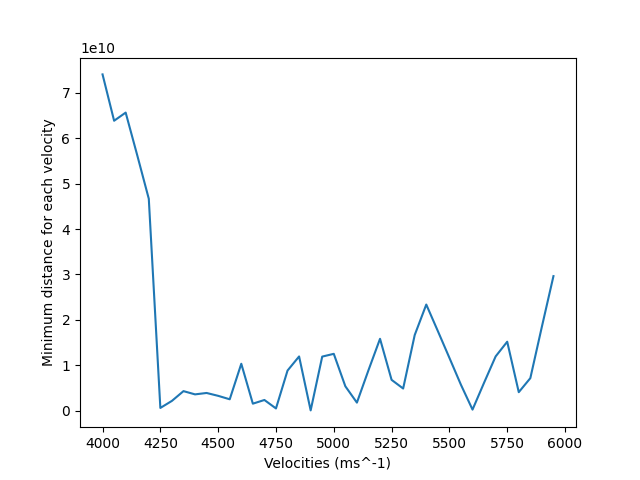
\includegraphics[width=6.40cm, height=4.80cm]{Full velocities medium survey.png}

    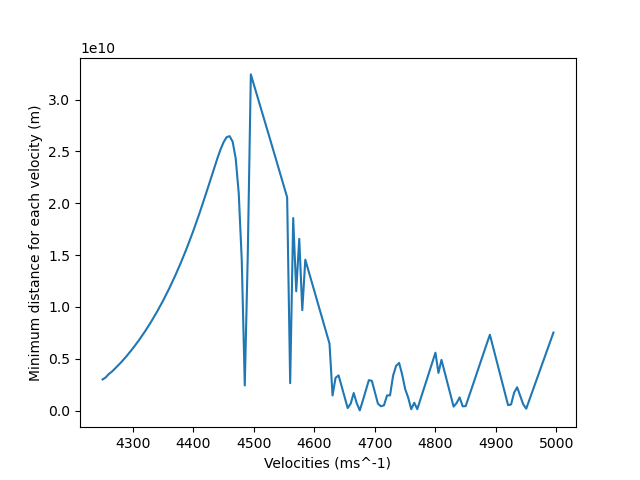
\includegraphics[width=6.40cm, height=4.80cm]{Velocity Big Survey.png}
    \caption{Graphics for the closest distance to mars for different velocities range. As the range of velocities decreases the number of different angles tested increases and the interval between velocities tested decreases.}
    \label{fig:my_label}

\end{figure}

{To determine the best velocity and angle of launch several surveys were made. Firstly a general survey with lower resolution (bigger interval between angles and velocities tested) for the expected velocity range ((0 to 10)$10^4$ $ms^{-1}$) and then further survey's into the areas which presented the smallest distances were made with an increasingly high resolution. The last graph shown on Figure 9 is the one with the highest resolution, testing velocities in intervals of 5$ms^{-1}$ and for every 4$^o$.}

{After all this the optimal velocity for the launch was found to be 4675$ms^{-1}$ and with a launch angle of 72$^o$. The satellite with this velocity would approach Mars at $2.69 * 10^7$ meters, which is very good since this simulation doesn't include the necessary manoeuvres that a satellite needs to do to enter a planet (that's the same reason why the satellite is assumed to already be in the orbit of the Earth). With these values the  will reach Mars approximately 1.194 years after its launch which is more than double of the perseverance arrival time of 7 months, or 0.58 years[3]. However, this is still within the expected time of one Mars period which is 1.862 years[1]. The Satellite will return to Earth (be within a $10^9$m order of magnitude of its centre of mass) after 10.74 years.}

{The results from this experience are very satisfactory since it manages to get a satellite closer to the centre of Mars than it was from the centre of the Earth at the beginning of its launch. However, these results are still constrained by computational limitations since the code that would run the simulation for all possible values of velocities for all possible angles of launch would take several days thus making it unrealistic to be executed for this project. However, the next step in this experiment would be using a higher resolution to make sure that there isn't a better angle capable of producing an even better-approaching distance to Mars.}

\section{Conclusion}

{In this experiment it was created a simulation of the Solar System in order to test its properties and potential factors that may influence it. }

{It was shown that the Beeman integration method is capable of predicting the periods of oscillation of the planets to a high degree of accuracy and conserves the energy of the system better than Euler's integration system. This allowed the conclusion that the Beeman integration method is the most suitable integration method to use in this simulation. }

{The effect of the rest of the planets' gravitational interactions was found to be negligible when compared with the gravitational effect of the Sun for relatively short time frames (30 years). }

{The optimal velocity to send a satellite to Mars was found to be 4675$ms^{-1}$ and with a launch angle of 72$^o$. The satellite reaches Mars 1.194 years after its launch and returns to Earth 10.74 years after the launch. }

{Overall the experiments were quite successful an the next steps in this projects would be expanding on experiments 2 and 4 in order test even more specific cases. }



\newpage

\section{References}

{Materials consulted during the elaboration of this report:}

{[1] https://nssdc.gsfc.nasa.gov/planetary/factsheet/planet\_table\_ratio.html consulted on 6/4/2023.}

{[2] Mohanna, Issam. (2020), "Precession of Mercury's Orbit in General Relativity and the Corrections to Newton's Gravitational Potential and Force" 10.13140/RG.2.2.31528.60164. }

{[3] https://mars.nasa.gov/mars2020/mission/faq/ consulted on 6/4/2023. }

{[4] Curtis, Howard, "Orbital Mechanics for Engineering Students", 2nd Edition, Butterworth-Heinemann, October 26, 2009. }




\end{document}
